\chapter{THE STANDARD MODEL} \label{sm}

The Standard Model (SM) of particle physics is an incredibly successful theory that correctly describes the physics of all known particles and forces that make up the universe \cite{smconsistency}. Well nearly all, quantum gravity and the non-zero neutrino mass are still a mystery \cite{smconsistency,smnograv,zee}. The particles of the SM come in two types: fermions and bosons. Fermions are the spin $\frac{1}{2}$ particles that make up the different types of matter, and bosons are the integer spin particles responsible for the different forces. Electrons are the most familiar type of fermion, but there are more exotic kinds like the quarks, neutrinos, muons, and the taus. The up and down quarks make up protons and neutrons, which combine to make nuclei, and nuclei combine with electrons to create the atoms that account for nearly all of the matter in our day to day experience. The up and down quarks and the electron are the first of three generations of quarks and leptons \footnote{Leptons are fermions like the electron that aren't quarks. The quarks interact with the strong force that binds nuclei together and the leptons do not.} with each generation heavier than the next. The up and down quarks are the first generation of quarks, charmed and strange are the next, and top and bottom are the third generation. For the leptons, the electron and electron neutrino are the first generation, the muon and muon neutrino are the second, and the tau and the tau neutrino the third. Each fermion also has a corresponding antiparticle. As an example, the positron is the antiparticle for the electron. 

\begin{figure}[h!]
  \centering
  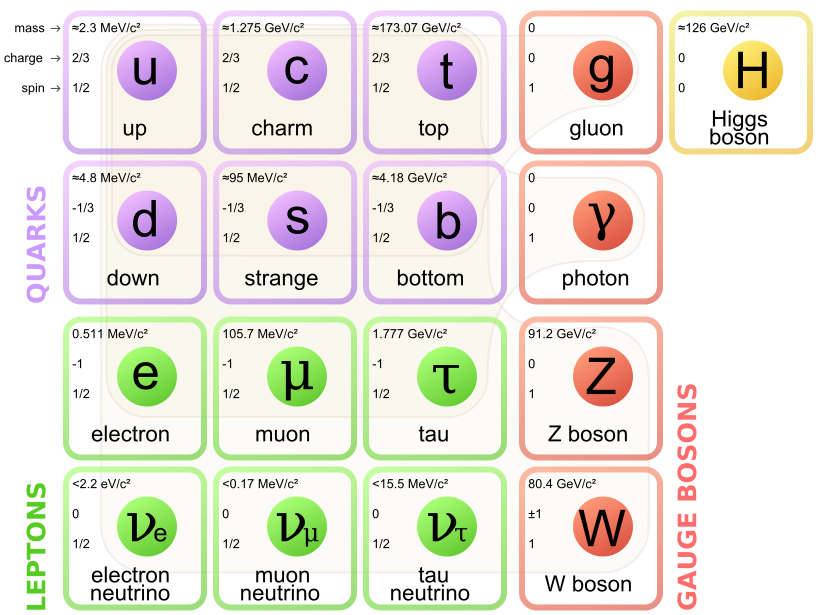
\includegraphics[width=4in]{images/Standard_Model_of_Elementary_Particles.png}
  \caption
   {The Standard Model Particles}
  \label{fig:smtable}
\end{figure}

The force carrying particles that allow matter to interact and form more complex objects like atoms, molecules, and even people are the spin 1 bosons. These force carriers are the gluons, photons, and the W and Z particles. Gluons mediate the strong force, photons the electromagnetic force, and the W and Z bosons mediate the weak force. Every force has an associated charge: particles with electric charge can interact through the electromagnetic force, those with color charge may interact via the strong force, and those with isospin or weak hypercharge may interact through the weak force. The fundamental forces bind the fermions to make the familiar composite objects that surround us. The strong force binds quarks into protons and neutrons and the protons and neutrons into nuclei, while the electromagnetic force binds the electrons and nuclei together to make atoms. The size of the composite objects gives an idea of the relative strength of the forces. A proton is ~$10^{-15}$ meters in size while an atom is ~$10^{-10}$ meters and a solar system is ~$10^{12}$ meters. The more tightly bound the stronger the force. But that isn't quite exact, in fact, the ratio of the strength of the forces is like so 1:$10^{-3}$:$10^{-16}$:$10^{-41}$, strong : electromagnetic : weak :gravitational \footnote{Gravity is just included for perspective. The Standard Model does not describe this force and reconciling gravity with quantum mechanics is an open problem.}. 

Of all the particles predicted by the SM, there is only one spin 0 particle, the Higgs boson, and it plays a special role in the theory. As the universe cooled from the Big Bang, the Higgs field went through a phase transition and settled into a nonzero ground state forming a condensate. The electron, muon, tau and the W and Z particles of the SM interact with the Higgs condensate and acquire mass. The massive particles of the SM are massively only because of the Higgs. With such a large role in the SM, finding this particle or a BSM Higgs has been a huge priority for the CMS collaboration \cite{tdr}. In 2012, a Higgs particle with a mass of 125 GeV was found and to date remains consistent with the Standard Model \cite{atlasdiscovery,cmsdiscovery2012,cmsdiscovery2013}. However, the properties need to be investigated further before declaring the discovered Higgs the Higgs of the Standard Model. 

The next sections build and couple the different Lagrangians to lay out the Standard Model and the Higgs mechanism. After putting the theory together, the more experimental details of the search for $H\rightarrow\mu^+\mu^-$ are described. In the following sections, $\hbar$ and the speed of light, c, are set to 1. Moreover, 0,1,2,3 and t,x,y,z are used interchangeably to label the components of a four vector. When relevant, 0 represents time and 1,2,3 represent x,y,z respectively. Einstein summation notation is used indicating that repeated indices are summed over, so $x_ix_i y_jy_j$ is shorthand for $\sum_i\sum_j x_ix_i y_jy_j$. Repeated Greek indices assume sums over all four space and time components, while repeated Roman indices assume sums over only the spatial components. 

%%%%%%%%%%%%%%%%%%%%%%%%%%%%%%%%%%
\section{QFT, Symmetries, and the Higgs Boson}

The laws of physics are invariant under boosts and rotations. Any proper QFT is described by an invariant Lagrangian respecting these symmetries. Boosts and rotations may be represented by different NxN matrices. The 4x4 matrices act on four vectors, the 2x2 matrices act on spinors, and the 1x1 matrices act on scalars. Scalars, four vector products, and certain spinor products remain invariant under Lorentz transformations so they are a natural ingredients for different QFTs. Scalar fields represent spin 0 particles, spinor fields represent spin 1/2 particles, and four vectors fields represent spin 1 particles. Coupling the spin 1 and spin 1/2 Lagrangians produces forces, and coupling the spin 1/2 and spin 1 fields to a spin 0 field produces mass. The spin 0 particle is the Higgs boson. In order to explain the Higgs coupling, the different Lagrangians are built and coupled. 

%%%%%%%%%%%%%%%%%%%%%%%%%%%%%%%%%%
\section{The Lagrangian for a Free Scalar Particle}

A scalar field remains the same under Lorentz transformations. This representation is used for spin 0 particles. The equations of motion must relate the change in the scalar field $\Phi$ at one moment in space and time to the value of $\Phi$ at the next moment in space and time, so the Lagrangian must include both the field itself and the four vector derivative, $\partial_\mu$. Note that both Newton's equations of motion, $F=m\ddot{x}$, and the Schrodinger equation for the free particle, $i\partial_t\psi = \frac{1}{2m}(-i\partial_x)(-i\partial_x)\psi$\footnote{Here the one dimensional case is presented for simplicity} have at most second order derivatives. The same holds for Maxwell's equations of electromagnetism. Hence, as an assumption, the derivative term in the Lagrangian will be the lowest order possible. As a Lorentz invariant scalar, any power of $\Phi$ can be included. On the other hand, $\partial_\mu$ is a four vector, and must be paired with a $\partial^\mu$ to form the invariant four vector product. Cross terms between these invariant pieces like $\Phi\partial_\mu\partial^\mu\Phi$ or $\partial_\mu\Phi\partial^\mu\Phi$ are also invariant, but lead to feedback between the derivatives and the value of the function. This means that the derivatives $i\partial_t = E$ and $-i\partial_i = P_i$ will change over time, but E and $\vec{P}$ should remain constant for a free particle. The cross terms are thrown out to prevent this. The $\Phi$ terms with an order different than $\Phi^2$ cause the same problem, and these are thrown out too. All of these choices lead to the following action, 
\begin{equation}
S = \int d^4x \left(c_0 + c_1 \Phi^2  
+ c_2 \partial_\mu\Phi\partial^\mu\Phi + c_3 \partial_\mu \partial^\mu \Phi\right).
\end{equation}

Note that the $c_3$ term is a total derivative and by the divergence theorem depends only on the values at the boundary, which are fixed. This implies that the contribution to the action from the $c_3$ term is the same regardless of how $\Phi$ changes in the volume. Because the Euler-Lagrange equations depend only on the variation in the volume, this term cannot contribute to $\delta S$ and $c_3$ may be set to zero. The $c_0$ term is a more obvious constant and does not affect $\delta S$ either, so it may be set to zero as well, leaving,  
\begin{equation}
S = \int d^4x \left(c_1 \Phi^2 + c_2 \partial_\mu\Phi\partial^\mu\Phi\right).
\end{equation}
Finding $\Phi$ such that $\delta S = 0$ amounts to applying the Euler-Lagrange equations $\partial_\mu \frac{\partial L}{\partial\left(\partial_\mu\Phi\right)} = \frac{\partial L}{\partial \Phi}$. These yield 
\begin{equation}
\begin{split}
&2c_2\partial_\mu\partial^\mu\Phi = -2c_1\Phi \\ 
&\rightarrow (-E^2 + \vec{P}^2)\Phi = \frac{c_1}{c_2}\Phi = -m^2\Phi \\
&\rightarrow \frac{c_1}{c_2} = -m^2.
\end{split}
\end{equation}

In order to get the correct dispersion relation for a relativistic particle, $c_1$ is set to $\frac{-1}{2}m^2$ and $c_2$ is set to $\frac{1}{2}$. Notice that including any $\Phi^n$ with n$\neq$2 in the Lagrangian would have contributed to the differential equation via $\frac{\partial L}{\partial \Phi}$ and that E, $\vec{P}$ wouldn't be constant. Thus the equation wouldn't work for a free particle. The resulting equation of motion for the scalar particle, $\partial_\mu\partial^\mu\Phi = -m^2\Phi$, is called the Klein-Gordon equation, and provides the correct description for spin 0 particles. This was all derived using symmetry, a reasonable assumption about the order of the derviatives, and the fact that the Energy shouldn't change over time for a free particle. The final Lagrangian for the scalar particle is 
\begin{equation}
S = \int d^4x \frac{1}{2}\left(\partial_\mu\Phi\partial^\mu\Phi - m^2 \Phi^2 \right).
\end{equation}

%%%%%%%%%%%%%%%%%%%%%%%%%%%%%%%%%%
\section{The Lagrangian for a Free Spin $\frac{1}{2}$ Particle}

With the action for the free scalar particle in hand, the free spin $\frac{1}{2}$ particle is up next. The spin $\frac{1}{2}$ action must combine the $\mathcal{L}$ (left-chiral) and $\mathcal{R}$ (right-chiral) spinors of the $(\frac{1}{2}, 0)$ and $(0, \frac{1}{2})$ representations and the four vector, $\partial_\mu$, in a Lorentz invariant way \cite{physymm}. The $\mathcal{L}$, $\mathcal{R}$, and $\partial_\mu$ transformations are now analyzed to find the lowest order invariant combinations. A Lorentz transformation for the left-chiral spinor is 
\begin{equation}
\Lambda^{(L)} = e^{\frac{i}{2}\theta_i \sigma_i + \frac{1}{2}\phi_i \sigma_i},
\end{equation}
and a Lorentz transformation for the right-chiral spinor is
\begin{equation}
\Lambda^{(R)} = e^{\frac{i}{2}\theta_i \sigma_i - \frac{1}{2}\phi_i \sigma_i}.
\end{equation}
Taking the Hermitian conjugate of the left-chiral transformation gives,
\begin{equation}
(\Lambda^{(L)})^\dagger = e^{-\frac{i}{2}\theta_i \sigma_i^\dagger + \frac{1}{2}\phi_i \sigma_i^\dagger} 
= e^{-\frac{i}{2}\theta_i \sigma_i + \frac{1}{2}\phi_i \sigma_i}.
\end{equation}
See Physics from Symmetry \cite{physymm} for more details. This reveals that $(\Lambda^{(L)})^\dagger$ is the inverse of $\Lambda^{(R)}$. Similarly, $(\Lambda^{(R)})^\dagger$ is the inverse of $\Lambda^{(L)}$. Thus, $\mathcal{L}^\dagger\mathcal{R}$ and $\mathcal{R}^\dagger\mathcal{L}$ are Lorentz invariants, which can be seen below,
\begin{equation}
(\mathcal{L}^\dagger\mathcal{R})' = \mathcal{L}^\dagger (\Lambda^{(L)})^\dagger \Lambda^{(R)} \mathcal{R} 
= \mathcal{L}^\dagger (\Lambda^{(R)})^{-1} \Lambda^{(R)} \mathcal{R} = \mathcal{L}^\dagger \mathcal{R}  
\end{equation}
\begin{equation}
(\mathcal{R}^\dagger\mathcal{L})' = \mathcal{R}^\dagger (\Lambda^{(R)})^\dagger \Lambda^{(L)} \mathcal{L} 
= \mathcal{R}^\dagger (\Lambda^{(L)})^{-1} \Lambda^{(L)} \mathcal{L} = \mathcal{R}^\dagger \mathcal{L}. 
\end{equation}
These are the lowest order invariant pieces involving the field alone. In order to couple the derivative to the field, the $\mathcal{L}$ and $\mathcal{R}$ spinors must attach to $\partial_\mu$ in an invariant way. A four vector may be expressed as an outer product of left and right spinors \cite{physymm}, 
\begin{equation}
\alpha_{L\tilde{R}} = \mathcal{L}_\alpha \tilde{\mathcal{R}}_\alpha^{T}.
\end{equation}
The following also works, 
\begin{equation}
\alpha_{R\tilde{L}} = \mathcal{R}_\alpha \tilde{\mathcal{L}}_\alpha^{T}.
\end{equation}
Combining left or right-chiral spinors with a $\sim$ provides a representation of a four vector that preserves the hermitivity and observability of a four vector operator. Unfortunately, the $\sim$ spinors add a bit of bookkeeping.

The $\sim$ transformation sends $\sigma_i$ to $-\sigma_i*$. So the transformations for the $\sim$ transposed spinors are,
\begin{equation}
(\Lambda^{(\tilde{L})})^T = e^{\frac{i}{2}\theta_i(-\sigma_i*)^T + \frac{1}{2}\phi_i (-\sigma_i*)^T} 
= e^{-\frac{i}{2}\theta_i \sigma_i^\dagger - \frac{1}{2}\phi_i \sigma_i^\dagger} = e^{-\frac{i}{2}\theta_i \sigma_i - \frac{1}{2}\phi_i \sigma_i}
\end{equation}
and
\begin{equation}
(\Lambda^{(\tilde{R})})^T = e^{\frac{i}{2}\theta_i(-\sigma_i*)^T - \frac{1}{2}\phi_i (-\sigma_i*)^T} 
= e^{-\frac{i}{2}\theta_i \sigma_i^\dagger + \frac{1}{2}\phi_i \sigma_i^\dagger} = e^{-\frac{i}{2}\theta_i \sigma_i + \frac{1}{2}\phi_i \sigma_i}.
\end{equation}
The equations above show that the $(\Lambda^{(\tilde{L})})^T$ transformation is the inverse of $\Lambda^{(L)}$, and that the $(\Lambda^{(\tilde{R})})^T$ transformation is the inverse of $\Lambda^{(R)}$. So the invariant pieces coupling the spinor to the four vector are,
\begin{equation}
\mathcal{R}^\dagger \alpha_{L\tilde{R}} \mathcal{R} = \mathcal{R}^\dagger \mathcal{L}_\alpha \tilde{\mathcal{R}}_\alpha^{T} \mathcal{R}
\end{equation}
and
\begin{equation}
\mathcal{L}^\dagger \alpha_{R\tilde{L}} \mathcal{L} = \mathcal{L}^\dagger \mathcal{R}_\alpha \tilde{\mathcal{L}}_\alpha^{T} \mathcal{L}.
\end{equation}
The two types of four vectors have slightly different transformations
\begin{equation}
\alpha_{L\tilde{R}}^{'} = e^{\frac{i}{2}\theta_i \sigma_i + \frac{1}{2}\phi_i \sigma_i} 
\alpha_{L\tilde{R}} e^{-\frac{i}{2}\theta_i \sigma_i + \frac{1}{2}\phi_i \sigma_i}
\end{equation}
\begin{equation}
\alpha_{R\tilde{L}}^{'} = e^{\frac{i}{2}\theta_i \sigma_i - \frac{1}{2}\phi_i \sigma_i} 
\alpha_{R\tilde{L}} e^{-\frac{i}{2}\theta_i \sigma_i - \frac{1}{2}\phi_i \sigma_i}.
\end{equation}
Both transform with positive $\theta$ under rotations, but the boosts are a different story. The $L\tilde{R}$ four vector transforms with positive $\phi$ while the $R\tilde{L}$ four vector transforms with negative $\phi$. The $R\tilde{L}$ rank 2 spinor is the parity flipped version of the $L\tilde{R}$ rank 2 spinor with negative spatial components:  
\begin{equation}
\begin{split}
&\alpha_{L\tilde{R}} = \alpha_0 \sigma_0 + \alpha_1 \sigma_1 + \alpha_2 \sigma_2 + \alpha_3 \sigma_3 \\
&\alpha_{L\tilde{R}} = \alpha_\mu \sigma^\mu \\
&\alpha_{L\tilde{R}} = 
\begin{pmatrix}
\alpha_0 + \alpha_3 & \alpha_1 - i\alpha_2 \\
\alpha_1 + i\alpha_2 & \alpha_0 - \alpha_3 \\
\end{pmatrix}
\end{split}
\end{equation}
versus
\begin{equation}
\begin{split}
&\alpha_{R\tilde{L}} = \alpha_0 \sigma_0 - \alpha_1 \sigma_1 - \alpha_2 \sigma_2 - \alpha_3 \sigma_3 \\
&\alpha_{R\tilde{L}} = \alpha_\mu \bar{\sigma}^\mu \\
&\alpha_{R\tilde{L}} = 
\begin{pmatrix}
\alpha_0 - \alpha_3 & \alpha_1 + i\alpha_2 \\
\alpha_1 - i\alpha_2 & \alpha_0 + \alpha_3 \\
\end{pmatrix}.
\end{split}
\end{equation}
The negative $\phi$ guarantees that the negative spatial components for a $R\tilde{L}$ rank 2 spinor add up with time the correct way in a boost.

The action for the spin $\frac{1}{2}$ particle is built from the lowest order invariant combinations of the spinors themselves and the lowest order invariant term coupling $\partial_\mu$ to the spinors. These ingredients are $\mathcal{L}^\dagger\mathcal{R}$, $\mathcal{R}^\dagger\mathcal{L}$, $\mathcal{R}^\dagger\sigma^\mu\partial_\mu\mathcal{R}$, and $\mathcal{L}^\dagger\bar{\sigma}^\mu\partial_\mu\mathcal{L}$. In the scalar particle case, m coupled the field to itself as potential energy with the same power as $\partial_\mu$ ($m^2\Phi^2\leftrightarrow\partial_\mu\Phi\partial^\mu\Phi$) \footnote{E, P, and m must have the same power to get $E^2 = m^2 + \vec{P}^2$ right, and $E \sim \partial_0$, $P_i \sim \partial_i$ so m must have the same power as $\partial_\mu$.}. Following that example and throwing an i into the derivative terms\footnote{The i gives the appropraite factor for the definition of $P_\mu$, $P_\mu = i\partial_\mu$.} to make them Hermitian gives the following Lagrangian,  
\begin{equation}
S = \int d^4x \left( \mathcal{R}^\dagger\sigma^\mu i\partial_\mu\mathcal{R} + i\mathcal{L}^\dagger\bar{\sigma}^\mu i\partial_\mu\mathcal{L} 
- m\mathcal{L}^\dagger\mathcal{R} - m\mathcal{R}^\dagger\mathcal{L} \right).
\end{equation} 
The Euler-Lagrange equations reveal how the fields change over time,
\begin{equation}
\begin{split}
& \sigma^\mu i\partial_\mu\mathcal{R} = m\mathcal{L} \\
& \bar{\sigma}^\mu i\partial_\mu\mathcal{L} = m\mathcal{R}. \\
& \sigma^\mu i\partial_\mu\mathcal{R}^\dagger = -m\mathcal{L}^\dagger \\
& \bar{\sigma}^\mu i\partial_\mu\mathcal{L}^\dagger = -m\mathcal{R}^\dagger. \\
\end{split}
\end{equation}
Notice that the mass term couples the left and right-chiral spinors. At rest, P=0 and the equations reduce to $i\partial_0\mathcal{R} = m\mathcal{L}$ and $i\partial_0\mathcal{L} = m\mathcal{R}$ showing that $\partial^2_0 \mathcal{R} = -m^2\mathcal{R}$ and $\partial^2_0 \mathcal{L} = -m^2\mathcal{L}$. The mass is actually a frequency determining how quickly a particle oscillates between its right-chiral and left-chiral states. Another interesting point is that swapping the sign of m here swaps the roles of the fields and the conjugate fields. 

Plugging $\mathcal{R} = \frac{1}{m}\bar{\sigma}^\nu i\partial_\nu\mathcal{L}$ into $\sigma^\mu i\partial_\mu\mathcal{R} = m\mathcal{L}$ shows that the constants chosen for the terms in the Lagrangian provide the correct dispersion relation,
\begin{equation}
\begin{split}
&\sigma^\mu i\partial_\mu \frac{1}{m}\bar{\sigma}^\nu i\partial_\nu\mathcal{L} = m\mathcal{L} \\
&\rightarrow \sigma^\mu \bar{\sigma}^\nu P_\mu P_\nu = m^2 \\
&\rightarrow \eta^\mu_\nu P_\mu P_\nu = m^2 \\
&\rightarrow P^\mu P_\mu = m^2 \\
&\rightarrow E^2 - \vec{P}^2 = m^2 \\
\end{split}
\end{equation}
The action for the spin $\frac{1}{2}$ particle can be rewritten into its more compact, canonical form,
\begin{equation}
S = \int d^4x \text{ } \bar{\psi} \left(i\gamma^\mu\partial_\mu - m\right)\psi,
\end{equation} 
after defining
\begin{equation}
\gamma^\mu =
\begin{pmatrix}
0 & \sigma^\mu \\
\bar{\sigma}^\mu & 0 \\
\end{pmatrix}
\text{, } 
\psi =
\begin{pmatrix}
\mathcal{L} \\
\mathcal{R} \\
\end{pmatrix}
\text{, and } 
\bar{\psi} =
\psi^\dagger \gamma_0 \text{. }
\end{equation}
The spin $\frac{1}{2}$ Lagrangian is called the Dirac Lagrangian and the resulting equations of motion are the Dirac equation.

%%%%%%%%%%%%%%%%%%%%%%%%%%%%%%%%%%
\section{The Lagrangian for a Free Spin 1 Particle}
Last but not least is the Lagrangian for a spin 1 force carrying particle. The main ingredients are the $A_\mu$ and $\partial_\mu$ four vectors. The lowest order possible invariants are $\partial^\mu A^\nu\partial_\mu A_\nu$, $\partial^\mu A^\nu\partial_\nu A_\mu$, $A^\mu A_\mu$, and $\partial^\mu A_\mu$. However the last term is a total derivative and won't be included. The resulting action and equations of motion are 
\begin{equation}
S = \int d^4x \left( c_0 i\partial^\mu A^\nu i\partial_\mu A_\nu + c_1 i\partial^\mu A^\nu i\partial_\nu A_\mu + c_2 A^\mu A_\mu \right).
\end{equation}
\begin{equation}
c_2 A^\nu = -\partial_\mu\left(c_0 \partial^\mu A^\nu + c_1 \partial^\nu A^\mu\right).
\end{equation}

This is the same form as the equation for the four vector potential in electromagnetism, which has $c_0 = \frac{1}{2}$ and $c_1 =-\frac{1}{2}$. The remaining term, $c_2$ looks like a mass term, so $c_2$ is set to $\frac{1}{2}m^2$ \footnote{The order of the mass should match the order of the derivatives.}. The action and equations of motion with the appropriate constants become, 
\begin{equation}
S = \int d^4x \left( \frac{-1}{2} \partial^\mu A^\nu\partial_\mu A_\nu + \frac{1}{2} \partial^\mu A^\nu\partial_\nu A_\mu + \frac{m^2}{2} A^\mu A_\mu \right)
\end{equation}
\begin{equation}
-m^2 A^\nu = \partial_\mu\left(\partial^\mu A^\nu - \partial^\nu A^\mu\right).
\end{equation}
Taking another derivative reveals that the equations reduce further and take on the correct dispersion relation, confirming the choice of constants,
\begin{equation}
\begin{split}
&-m^2 \partial_\nu A^\nu = \partial_\nu \partial_\mu \partial^\mu A^\nu - \partial_\nu \partial_\mu \partial^\nu A^\mu = 0 \\
&\rightarrow \partial_\nu A^\nu = 0 \\
&\rightarrow -m^2 A^\nu = \partial_\mu\partial^\mu A^\nu \\
&\rightarrow m^2 A^\nu = i\partial_\mu i\partial^\mu A^\nu \\
&\rightarrow m^2 = E^2 - \vec{P}^2.
\end{split}
\end{equation}
The action for the spin 1 particle is called the Proca action. It's normally written in an equivalent form in terms of the tensor $F_{\mu\nu} = \partial_\mu A_\nu - \partial_\nu A_\mu$
\begin{equation}
S = \int d^4x \left( \frac{-1}{4}F_{\mu\nu}F^{\mu\nu}  + \frac{m^2}{2} A^\mu A_\mu \right).
\end{equation}


%%%%%%%%%%%%%%%%%%%%%%
\section{Interactions}

In order to describe theories where fermions and bosons interact, the spin 1 and spin 1/2 are coupled. The simplest Lorentz invariant term that couples a vector to the Dirac spinors is $\bar{\psi}\gamma^\mu A_\mu \psi$, providing an interacting theory that looks like 
%Massive QED
\begin{equation}
\begin{split}
S &= \int d^4x \frac{-1}{4}F_{\mu\nu}F^{\mu\nu} + \frac{m_A^2}{2} A^\mu A_\mu + \bar{\psi}\left(i\gamma^\mu\partial_\mu - m\right)\psi + q\bar{\psi}\gamma^\mu A_\mu \psi \\
&= \int d^4x \frac{-1}{4}F_{\mu\nu}F^{\mu\nu} + \frac{m_A^2}{2} A^\mu A_\mu + \bar{\psi}\left[i\gamma^\mu\left(\partial_\mu - iqA_\mu\right)- m \right]\psi. 
\end{split}
\end{equation}
To describe electromagnetism, the photon field should be massless and the theory should be gauge invariant. Setting $m_A$ to zero and checking whether $A_\mu \rightarrow A_\mu(x) + \partial_\mu\alpha(x)$ is a symmetry, provides  
%S = \int d^4x \frac{-1}{4}F_{\mu\nu}F^{\mu\nu} + \bar{\psi}\left(i\gamma^\mu\partial_\mu - m + q\gamma^\mu A_\mu + q\gamma^\mu\partial_\mu\alpha\right)\psi.
\begin{equation}
S = \int d^4x \frac{-1}{4}F_{\mu\nu}F^{\mu\nu} + \bar{\psi}\left[i\gamma^\mu\left(\partial_\mu - iqA_\mu - iq\partial_\mu\alpha\right)- m \right]\psi, 
\end{equation}
which isn't gauge invariant. In effect, the gauge transformation on $A_\mu$ has shifted the derivative, $\partial_\mu \rightarrow \partial_\mu - iq\partial_\mu\alpha$. In order to retain gauge invariance, a simultaneous transformation that sends $\partial_\mu \rightarrow \partial_\mu + iq\partial_\mu\alpha$ is needed to cancel out the extra term. The correct transformation is $\bar{\psi}\partial_\mu\psi \rightarrow \bar{\psi} e^{-iq\alpha} \partial_\mu e^{iq\alpha} \psi$. So, if 
\begin{equation}
A_\mu(x) \rightarrow A_\mu(x) + \partial_\mu\alpha(x)
\end{equation}
and
\begin{equation}
\psi(x) \rightarrow e^{iq\alpha(x)}\psi(x) 
\end{equation}
the Lagrangian is gauge invariant. The second equation reveals that the field is invariant under local transformations of the phase. 

Requiring gauge invariance requires the fermion field to maintain U(1) invariance. By running the logic in reverse and demanding more complicated unitary invariances on the fermion field(s), Lagrangians may be produced that describe new forces. In the case of electromagnetism above, demanding that the fermion field is invariant under a local U(1) transformation, sends $\bar{\psi}\partial_\mu\psi \rightarrow \bar{\psi} e^{-iq\alpha} \partial_\mu e^{iq\alpha} \psi$ effectively shifting the derivative, $\partial_\mu \rightarrow \partial_\mu + iq\partial_\mu\alpha$. Now $A_\mu$ needs to cancel the shift requiring 

\begin{equation}
\partial_\mu + iq\partial_\mu\alpha + c(A_\mu + a_\mu) = \partial_\mu + cA_\mu. 
\end{equation}
Therefore c=-iq and $a_\mu = \partial_\mu\alpha$. Furthermore, $F^{\mu\nu}F_{\mu\nu}$ must remain invariant under $A_\mu(x) \rightarrow A_\mu(x) + \partial_\mu\alpha(x)$. These conditions plus Lorentz invariance force the Lagrangian to be of the form, 
\begin{equation}
S = \int d^4x \frac{-1}{4}(\partial_\mu A_\nu - \partial_\nu A_\mu)(\partial^\mu A^\nu - \partial^\nu A^\mu) + \bar{\psi}\left[i\gamma^\mu\left(\partial_\mu - iqA_\mu\right) - m \right]\psi, 
\end{equation}
which correctly describes Quantum Electrodynamics (QED) \cite{zee}.

The QED U(1) symmetry has a single generator and, as a consequence, bypasses any commutation issues. The SU(2) transformation $\psi \rightarrow U\psi$ with $U = e^{\frac{i}{2}q\alpha_i(x)\sigma_i}$ is a bit more complicated. For any unitary transformation, if 
\begin{equation}
\bar{\psi}U^\dagger i\gamma^\mu\left(\partial_\mu + cA'_{\mu}\right)U\psi = \bar{\psi}i\gamma^\mu\left(\partial_\mu + cA_{\mu}\right)\psi 
\end{equation}
is true when $A_\mu \rightarrow A'_\mu$, then by definition gauge invariance is retained. This is true when $\left(\partial_\mu + cA'_{\mu}\right)U\psi =U\left(\partial_\mu + cA_{\mu}\right)\psi$. Breaking down the transformation on $A_{\mu}$ into $A_\mu \rightarrow UA_\mu U^\dagger + \Delta A_{\mu}$ helps simplify the conditions for gauge invariance, 
\begin{equation}
\begin{split}
\left(\partial_\mu + cA'_{\mu}\right)U\psi &=  \partial_\mu(U\psi) + cA'_{\mu}U\psi \\
& = (\partial_\mu U)\psi + U(\partial_\mu\psi) + cA'_{\mu}U\psi \\ 
& = (\partial_\mu U)\psi + U(\partial_\mu\psi) + cUA_{\mu}U^\dagger U\psi + c\Delta A_{\mu}U\psi \\
& = U\left(\partial_\mu + cA_{\mu}\right)\psi + (\partial_\mu U)\psi + c\Delta A_{\mu}U\psi.
\end{split}
\end{equation}
To get $U\left(\partial_\mu + cA_{\mu}\right)\psi$ and retain invariance, $(\partial_\mu U)\psi + c\Delta A_{\mu}U\psi$ must be zero. This requires 
\begin{equation}
c\Delta A_{\mu}U\psi = -(\partial_\mu U)\psi = - (\partial_\mu U)U^\dagger U\psi = U(\partial_\mu U^\dagger) U\psi.
\end{equation}
The last line uses the fact that for a unitary matrix U, $UU^\dagger = 1$ and $\partial_\mu(UU^\dagger) = 0$. Therefore, to preserve gauge invariance under the unitary transformation $\psi \rightarrow U\psi$, $cA_\mu$ must transform as
\begin{equation}
cA_\mu(x) \rightarrow cUA_\mu(x)U^\dagger + U\partial_\mu U^\dagger .
\end{equation}
For invariance under SU(2) the derivative can be calculated explicitly
\begin{equation}
\begin{split}
cA_\mu(x) &\rightarrow cUA_\mu(x)U^\dagger + c\Delta A_\mu \\ 
&= cUA_\mu(x)U^\dagger - iq\frac{\sigma_i}{2}\partial_\mu\alpha_i(x).
\end{split}
\end{equation}
Choosing c=-iq and $\Delta A_\mu = \frac{\sigma_i}{2}\partial_\mu\alpha_i(x)$ determines the coupling constant and the transformation for the SU(2) invariant Lagrangian.

$A_\mu$ is a matrix which may be expanded in terms of the SU(2) generators, $A_\mu$ = $A^1_{\mu}\frac{\sigma_1}{2}$ + $A^2_{\mu}\frac{\sigma_2}{2}$ + $A^3_{\mu}\frac{\sigma_3}{2}$. Note that U(1) only requires a single particle while SU(2) requires three. For the SU(N) transformations, there will be a force carrying particle for each generator, and the field may be expanded using the generators as a basis, $A_\mu = T^cA^c_\mu$. In this case, the transformation for each component of $A_\mu$ may be written explicitly, 
\begin{equation}
\label{eq:Agauge}
A^c_\mu \rightarrow A^c_\mu - f^{abc}\alpha^a A^b_\mu + \partial_\mu\alpha^c, 
\end{equation}
where $[T^a,T^b]=if^{abc}T^c$ defines the Lie alegbra of the group. For SU(2) in particular, $A_\mu = \frac{\sigma_c}{2}A^c$ and $f^{abc} = \epsilon^{abc}$.
This defines half of the SU(2) Lagrangian, but $F_{\mu\nu}$ still needs to be defined so that it remains invariant under equation \ref{eq:Agauge}. Defining 
\begin{equation}
F_{\mu\nu} = \partial_\mu A_\nu - \partial_\nu A_\mu - iq[A_\mu,A_\nu] 
\end{equation}
makes $F_{\mu\nu}$ covariant, $F_{\mu\nu} \rightarrow UF_{\mu\nu}U^\dagger$, \cite{zee} and to make it invariant, the trace is taken. So finally, the full gauge invariant Lagrangian with massless fermions is given by
\begin{equation}
S = \int d^4x \mathcal{N}tr(F_{\mu\nu}F^{\mu\nu}) + \bar{\psi}i\gamma^\mu D_\mu\psi,
\end{equation}
where $D_\mu = \partial_\mu - iqA_\mu$ is the covariant derivative. The Lagrangian holds for the U(1) and SU(N) gauge transformations. U(1) provides electromagnetism, adding on SU(2) provides the electroweak interactions, and adding SU(3) provides the strong force. All three together, describe the Standard Model. Writing out the trace in terms of the generators, the Lagrangian is given by, 
\begin{equation}
\label{eq:ewlagrangian}
S = \int d^4x \frac{-1}{2}tr(F_{\mu\nu}F^{\mu\nu}) + \bar{\psi}i\gamma^\mu D_\mu\psi 
  = \int d^4x \frac{-1}{4}F^a_{\mu\nu}F_a^{\mu\nu} + \bar{\psi}\left[i\gamma^\mu\left(\partial_\mu - iqT^iA^i_\mu\right)\right]\psi. 
\end{equation}
where
\begin{equation}
F^a_{\mu\nu} = \partial_\mu A^a_\nu - \partial_\nu A^a_\mu + qf^{abc}A^b_\mu A^c_\nu. 
\end{equation}
$\mathcal{N}$ is set to $-\frac{1}{2}$ in order to get the appropriate $-\frac{1}{4}$ in front of the $F^a_{\mu\nu}$ tensors\footnote{The calculation uses the fact that the SU(N) the generator matrices form an orthogonal basis, $tr(T^aT^b) = \frac{1}{2}\delta^{ab}$.}.

The SU(2) invariant Lagrangian of equation \ref{eq:ewlagrangian} provides the weak interaction. Unfortunately, the theory has massless fermions and massless weak force particles, while in real life these particles have mass. Adding mass terms directly ruins the SU(2) invariance, so another mechanism is needed, and this is where the Higgs comes into play.  
%= \int d^4x \frac{-1}{4}F^a_{\mu\nu}F_a^{\mu\nu} + \bar{\psi}i\gamma^\mu D_\mu\psi,
%\underbracket[0.8pt]{\mathcal{D}_F(x_2,x_1)}_\text{A}
%iq\frac{\sigma_i}{2}\partial_\mu\alpha_i
%\begin{equation}
%\bar{\psi}U^\dagger i\gamma^\mu\left(\partial_\mu + iq\frac{\sigma_i}{2}\partial_\mu\alpha_i + c_i(A_{i\mu} + a_{i\mu})\right)U\psi 
%= \bar{\psi}i\gamma^\mu\left(\partial_\mu + cA_{i\mu}\right)\psi, 
%\end{equation}

%%%%%%%%%%%%%%%%%%%%%%
\section{The Higgs Mechanism}
The W and Z bosons observed in nature are massive, but directly adding a mass term for a force carrying particle ruins the gauge symmetry, 
\begin{equation}
\frac{1}{2}m_A^2A_\mu A^\mu \rightarrow \frac{1}{2}m_A^2(UA_\mu U^\dagger + \Delta A_\mu)(UA^\mu U^\dagger + \Delta A^\mu). 
\end{equation}
Both the  $UAU^\dagger$ and the $\Delta A$ are a problem. Meanwhile for the matter particles, the gauge transformation acts on a column of fermions which leaves the $\bar{\psi}m\psi$ term invariant,  
\begin{equation}
\begin{pmatrix}
\bar{\psi_1} \\
...          \\
\bar{\psi_n} \\
\end{pmatrix}
m
\begin{pmatrix}
\psi_1 & ... & \psi_n
\end{pmatrix}
\rightarrow
\begin{pmatrix}
\bar{\psi_1} \\
...          \\
\bar{\psi_n} \\
\end{pmatrix}
U^\dagger mU
\begin{pmatrix}
\psi_1 & ... & \psi_n
\end{pmatrix},
\end{equation}
but this term restricts the fermions to the same mass. In order to describe the massive fermions and the massive W and Z particles seen in nature the Higgs mechanism is needed. Relativistically, mass is energy, so the idea is to produce $m_A^2A_\mu A^\mu$ and $\bar{\psi}m\psi$ terms via some interaction energy involving a new field. Because mass is a scalar, the interactions require a scalar field, and because the mass is derived from a nonzero interaction energy, the groundstate of the scalar field should be nonzero. For all of these reasons, the Higgs mechanism adds a scalar field with a $\phi^4$ potential term to the Lagrangian, 
\begin{equation}
\label{eq:toyew1}
\mathcal{L}^{toy}_\phi = (\partial^\mu\phi - iqA^\mu\phi)^\dagger(\partial_\mu\phi - iqA_\mu\phi) + \frac{m_h^2}{2}\phi^\dagger\phi - \frac{\lambda}{4}(\phi^\dagger\phi)^2.
\end{equation}
As $\phi$ goes into the groundstate, $\phi \rightarrow \phi_0$, the force carrying field(s) acquire mass through the $A^2\phi_0^2$ terms. Similarly, interaction terms coupling the left and right spinors provide the fermions with mass as $\phi \rightarrow \phi_0$
\begin{equation}
\label{eq:toyew2}
\mathcal{L}^{toy}_I = -\beta(L^\dagger\phi R + R^\dagger\phi L).
\end{equation}

The toy examples of equations \ref{eq:toyew1} and \ref{eq:toyew2} cover the basic ideas behind the Higgs mechanism, but correctly describing the electroweak interaction requires a more complex and intricate theory, the U(1)xSU(2) Weinberg-Salam Lagrangian. The Weinberg-Salam Lagrangian includes a U(1) gauge field and an SU(2) gauge field. In the theory, the U(1) field and the third component of the SU(2) field mix up, with one orthogonal piece providing the massive Z boson and the other the massless photon. The remaining first and second components of the SU(2) field mix up to provide the massive $W^+$ and $W^-$ bosons. 

The Weinberg-Salam Lagrangian for the electron (e) and electron neutrino ($\nu_e$) of equation \ref{eq:ws} is written in terms of left and right handed Dirac spinors, $e_L$, $e_R$, and $\nu_e$. Left and right handed Dirac spinors for a particle are defined in terms of the left and right handed spinors (s) for the particle as follows, $\psi_L = \begin{pmatrix} s_L \\ 0 \end{pmatrix}$ and $\psi_R = \begin{pmatrix} 0 \\ s_R \end{pmatrix}$. In nature, the weak force treats left and right handed particles differently. The $W^+$ and $W^-$ particles interact only with left handed particles and interact with those of the same generation symmetrically. To respect this symmetry, the Lagrangian is written to respect the interchange of the left handed, same generation particles. The left swapping symmetry is an SU(2) transformation acting on the column vector of left handed Dirac spinors, $L = \begin{pmatrix} \nu_e \\ e_L \end{pmatrix}$. The remaining right handed particle is denoted by $R = e_R$. In addition, only left handed neutrinos have been observed in nature, so $\nu_e$ is left handed. The electroweak Lagrangian is then,  
\begin{equation}
\label{eq:ws}
\begin{split}
\mathcal{L} &= (\partial^\mu\phi - iq_{w\phi}\frac{\sigma_i}{2}W_i^\mu\phi - iq_{b\phi}B^\mu\phi)^\dagger
               (\partial_\mu\phi - iq_{w\phi}\frac{\sigma_i}{2}W^i_\mu\phi - iq_{b\phi}B^\mu\phi) \\ 
            &+ \bar{L}i\gamma^\mu(\partial_\mu - iq_{wl}\frac{\sigma_i}{2}W_i^\mu - iq_{bl}B_\mu)L + \bar{R}i\gamma^\mu(\partial_\mu - iq_{br}B_\mu)R \\
            &- \beta(\bar{\nu}_e\phi_+e_R + \bar{e}_R\phi_+^{*}\nu_e + \bar{e}_L\phi_-e_R + \bar{e}_R\phi_-^{*}e_L) 
             - \frac{1}{4}G_i^{\mu\nu}G^i_{\mu\nu} -\frac{1}{4}F^{\mu\nu}F_{\mu\nu} \\
            &+ \frac{m_h^2}{2}\phi^\dagger\phi - \frac{\lambda}{4}(\phi^\dagger\phi)^2.
\end{split}
\end{equation}
The SU(2) field, $W_\mu$, in its simplest nontrivial representation is a complex 2x2 matrix that operates on 2x1 complex column vectors. Therefore $\phi$ is written 
\begin{equation}
\phi = 
\begin{pmatrix}
\phi_+ \\ \phi_-
\end{pmatrix}.
\end{equation}
To isolate the mass terms, the scalar field is expanded about its minimum, $|\phi_{min}| = \phi_0 = \sqrt{\frac{m_h^2}{\lambda}}$. The minimum is degenerate, only requiring that $|\phi_+|^{2} + |\phi_-|^{2} = \phi_0^2$. The particular solution $\phi = \begin{pmatrix} 0 \\ \phi_0 + \frac{1}{\sqrt{2}}h(x) \end{pmatrix}$ fixes the fermion mass terms such that the electron acquires mass in the correct way. The choice also eliminates the strange mass-like coupling between the electron and neutrino,
\begin{equation}
\beta(\bar{L}\phi R + \bar{R}\phi^\dagger L) = \beta(\bar{\nu}_e\phi_+e_R + \bar{e}_R\phi_+^{*}\nu_e + \bar{e}_L\phi_-e_R + \bar{e}_R\phi_-^{*}e_L) \rightarrow 
\beta(\bar{e}_L\phi_0e_R + \bar{e}_R\phi_0e_L).
\end{equation}
Fixing $\phi^+=0$ and $Im\phi^-=0$ comes at a cost, breaking the SU(2) symmetry of the Lagrangian. The coupling is no longer in the invariant form $\bar{L}\phi R + \bar{R}\phi^\dagger L \rightarrow \bar{L}U^\dagger U\phi R + \bar{R}\phi^\dagger U^\dagger UL$. 

As in the toy example, the $(D^\mu\phi)^\dagger(D_\mu\phi)$ term bestows mass onto the force carriers,
\begin{equation}
\begin{split}
D_\mu\phi &= (\partial_\mu - iq_{w\phi}\frac{\sigma_i}{2}W^i_\mu - iq_{b\phi}B_\mu)\phi \\
          &= \left[ 
\begin{pmatrix}
\partial_\mu - iq_{b\phi}B_\mu & 0 \\
0 & \partial_\mu - iq_{b\phi}B_\mu \\
\end{pmatrix} 
 - \frac{i}{2}q_{w\phi}
\begin{pmatrix}
W^3_\mu & W^1_\mu - iW^2_\mu \\
W^1_\mu + iW^2_\mu & -W^3_\mu \\
\end{pmatrix} \right] \begin{pmatrix} 0 \\ \phi_0 + \frac{1}{\sqrt{2}}h \end{pmatrix} \\
%          &=
%\begin{pmatrix} 0 \\ \frac{1}{\sqrt{2}}\partial_\mu h - iq_{b\phi}B_\mu(\phi_0 + \frac{1}{\sqrt{2}}h) \end{pmatrix}
% - \frac{i}{2}q_{w\phi}
%\begin{pmatrix}
%(W^1_\mu - iW^2_\mu)(\phi_0 + \frac{1}{\sqrt{2}}h)\\
%-W^3_\mu(\phi_0 + \frac{1}{\sqrt{2}}h) \\
%\end{pmatrix} \\ 
%         &= -\frac{i}{2}
%\begin{pmatrix}
%q_{w\phi}(W^1_\mu - iW^2_\mu)(\phi_0 + \frac{1}{\sqrt{2}}h)\\
%i\sqrt{2}\partial_\mu h - q_{w\phi}W^3_\mu(\phi_0 + \frac{1}{\sqrt{2}}h) + 2q_{b\phi}B_\mu(\phi_0 + \frac{1}{\sqrt{2}}h)\\
%\end{pmatrix} \\
         &= -\frac{i}{2}
\begin{pmatrix}
q_{w\phi}\phi_0(W^1_\mu - iW^2_\mu) + \frac{1}{\sqrt{2}}q_{w\phi}h(W^1_\mu - iW^2_\mu)\\
i\sqrt{2}\partial_\mu h + \phi_0(2q_{b\phi}B_\mu - q_{w\phi}W^3_\mu) + \frac{1}{\sqrt{2}}h(2q_{b\phi}B_\mu - q_{w\phi}W^3_\mu)\\
\end{pmatrix}.
\end{split}
\end{equation}
The $\phi_0^2$ terms determine the masses,
\begin{equation}
(D^\mu\phi)^\dagger(D_\mu\phi) = q^2_{w\phi}\frac{\phi_0^2}{4}(W^1_\mu)^2 + q^2_{w\phi}\frac{\phi_0^2}{4}(W^2_\mu)^2 
                                      + \frac{\phi_0^2}{4}(q_{w\phi}W^3_\mu - 2q_{b\phi}B_\mu)^2 + \text{other terms.}
\end{equation}
The orthogonal term $q_{w\phi}W^3_\mu + 2q_{b\phi}B_\mu$ is missing from the covariant derivative and remains massless \cite{qftam}, providing the photon field. This leaves 
\begin{equation}
m_{w} = \frac{q_{w\phi}\phi_0}{\sqrt{2}} \text{, }
m_z = \frac{m_w}{q_{w\phi}} \text{, and } m_\gamma = 0.
\end{equation}
The photon, $A_\mu$, is a linear combination of $W^3_\mu$ and $B_\mu$, which implies that the U(1) symmetry corresponding to electromagnetism is also a linear combination, 
\begin{equation}
\begin{split}
& U_A = e^{i(Q_{wi}T^3 + Q_{bi})\alpha(x)}, \\
& W^3_\mu \rightarrow W^3_\mu + \frac{1}{g_w}\partial_\mu\alpha, \\
& B_\mu \rightarrow B_\mu + \frac{1}{g_b}\partial_\mu\alpha.
\end{split}
\end{equation}
$T^3$ is the third SU(2) generator for the given representation, and the Qs are the normalized charges defined by,
\begin{equation}
q_{wi} = Q_{wi}g_w \text{ and } q_{bi} = Q_{bi}g_b.
\end{equation} 
The U(1) gauge symmetry leads to conservation of electromagnetic charge, $Q = Q_{w}I_{3} + Q_{b}$, implying that the electromagnetic charge for a given particle is $Q_i = Q_{wi}I_{3i} + Q_{bi}$. $I_{3i}$ represents the eigenvalue of the $T^3$ generator denoting the particle eigenstate. For example, the operator $T^3 = \frac{\sigma^3}{2}$ acting on L has two eigenstates, $\nu_e$ and $e_L$, corresponding to eigenvalues $I_{3\nu_e} = \frac{1}{2}$ and $I_{3e_L} = \frac{-1}{2}$ respectively. Similarly, the eigenstates $\phi^+ = 0$ and $\phi^- = \phi_0 + h$ correspond to eigenvalues $I_{3\phi^+} = \frac{1}{2}$ and $I_{3\phi^-} = \frac{-1}{2}$.  

The symmetry of the W particles towards the left handed particles implies that the left handed particles have the same charge, $Q_{wi} = 1$. The lack of interaction between the W paricles and the right handed particles implies that the right handed particles have $Q_{wi} = 0$. The Higgs is assumed to interact with the W particles the same way as the left handed ones with a $Q_{wi} = 1$. The electromagnetic charge $Q_i$ and the isospin $Q_{wi}$ values fix the remaining electroweak $Q_{bi}$ values, 
\begin{equation}
\begin{split}
&Q_{e_L} = Q_{we_L}I_{3e_L} + Q_{be_L} = \frac{-1}{2} + Q_{be_L} \\
&Q_{e_R} = Q_{we_R}I_{3e_R} + Q_{be_R} = 0 + Q_{be_R} \\
&Q_{\nu_e} = Q_{w\nu_e}I_{3\nu_e} + Q_{b\nu_e} = \frac{1}{2} + Q_{b\nu_e} \\
&Q_{\phi^-} = Q_{w\phi^-}I_{3\phi^-} + Q_{b\phi^-} = \frac{-1}{2} + Q_{b\phi^-},
\end{split}
\end{equation}
providing, 
\begin{equation}
Q_{be_L} = \frac{-1}{2}\text{, } Q_{be_R} = -1 \text{, } Q_{b\nu_e} = \frac{-1}{2} \text{, and } Q_{b\phi^-} = \frac{+1}{2}.
\end{equation}
The electroweak Lagrangian reduces to,
\begin{equation}
\label{eq:ewlred}
\begin{split}
\mathcal{L} &= (\partial^\mu\phi - ig_{w}\frac{\sigma_i}{2}W_i^\mu\phi - \frac{i}{2}g_{b}B^\mu\phi)^\dagger
               (\partial_\mu\phi - ig_{w}\frac{\sigma_i}{2}W^i_\mu\phi - \frac{i}{2}g_{b}B^\mu\phi) \\ 
            &+ \bar{L}i\gamma^\mu(\partial_\mu - ig_{w}\frac{\sigma_i}{2}W_i^\mu + \frac{i}{2}g_{b}B_\mu)L + \bar{R}i\gamma^\mu(\partial_\mu + ig_{b}B_\mu)R \\
            &- \beta(\bar{L}\phi R + \bar{R}\phi^\dagger L) 
             - \frac{1}{4}G_i^{\mu\nu}G^i_{\mu\nu} -\frac{1}{4}F^{\mu\nu}F_{\mu\nu} + \frac{m_h^2}{2}\phi^\dagger\phi - \frac{\lambda}{4}(\phi^\dagger\phi)^2,
\end{split}
\end{equation}
with $\phi = \begin{pmatrix} 0 \\ \phi_0 + \frac{1}{\sqrt{2}}h(x) \end{pmatrix}$ and $L = \begin{pmatrix} \nu_e \\ e_L \end{pmatrix}$. In equation \ref{eq:ewlred}, the $W^+$ particle is $W^1_\mu+iW^2_\mu$, and the $W^-$ particle is $W^1_\mu - iW^2_\mu$. The photon is $g_{w}W^3_\mu + g_{b}B_\mu$, the Z boson is $g_{w}W^3_\mu - g_{b}B_\mu$, and the Higgs boson is h(x). Adding the next two generations of leptons, the three generations of quarks, and the SU(3) interactions to the electroweak Lagrangian defines the entire Standard Model.   
%\begin{pmatrix} 0 \\ \phi_0 + \frac{1}{\sqrt{2}}h \end{pmatrix}
%Only left handed neutrinos have been observed in nature, so the electron neutrino in the Lagrangian is a left handed Dirac spinor.
% The left handed Dirac spinors are concatenated into $L = \begin{pmatrix} \nu_e \\ e_L \end{pmatrix}$.
%Left and right Dirac spinors are defined in terms of the left and right spinors as follows, $\psi_L = \begin{pmatrix} L 0 \end{pmatrix}$ and $\psi_R = \begin{pmatrix} 0 R \end{pmatrix}$. Note that the neutrino is purely left handed as verified by experiment.

%%%%%%%%%%%%%%%%%%%%%%%%%%%%%%%%%%
%\section{Calculating QFT: Feynman Diagrams}
%
%In general the amplitude to go from a state $\phi(t_0) = \phi_0$ to $\phi(t_f) = \phi_f$ is determined by the sum over all possible paths, 
%\begin{equation}
%\mathcal{A}(\phi_f, t_f; \phi_0, t_0) = \braket{\phi_f,t_f|\phi_0,t_0} = \int \mathcal{D}[\cdot] e^{i\int_{t_0}^{t_f} dt L}.
%\end{equation}
%Furthermore, the expectation value for an operation performed at time $t_1$ when the system starts in the state $\phi(t_0) = \phi_0$ and ends in $\phi(t_f) = \phi_f$ is
%\begin{equation}
%|\bra{\phi_f,t_f}\mathcal{O}(t_1)\ket{\phi_0,t_0}|^2 = \left|\int \mathcal{D}[\cdot] \mathcal{O}(t_1) e^{i\int_{t_0}^{t_f} dt L}\right|^2.
%\end{equation}
%Of particular importance for QFT are scattering events. When two particles are measured at $(t_1,\vec{x}_1)$ and $(t_2,\vec{x}_2)$ some time in the past, what is the amplitude to measure two particles at $(t_3,\vec{x}_3)$ and $(t_4,\vec{x}_4)$ some time in the future? Considering that particles are excitations of a field, an equivalent question may be asked. How is the field amplitude correlated between spacetime points $(t_4, \vec{x}_4), (t_3, \vec{x}_3), (t_2, \vec{x}_2),$ and $(t_1, \vec{x}_1)$ \cite{zee}. For two to two scattering the amplitude is given by
%\begin{equation}
%\bra{0}\psi_i(t_4,\vec{x}_4)\psi_j(t_3,\vec{x}_3)\psi_k(t_2,\vec{x}_2)\psi_l(t_1,\vec{x}_1)\ket{0} = 
%\frac{\int \mathcal{D}[\cdot]\psi_i(t_4,\vec{x}_4)\psi_j(t_3,\vec{x}_3)\psi_k(t_2,\vec{x}_2)\psi_l(t_1,\vec{x}_1)
%e^{i\int_{-\infty}^{\infty} dt L}}{\int \mathcal{D}[\cdot]e^{i\int_{-\infty}^{\infty} dt L}},
%\end{equation}
%where $\psi$ is a field, 0 denotes the vacuum state, and i, j, k, l specify the types of particles observed \cite{peskin}. Calculating this path integral for the full Lagrangian determines the amplitude for the scattering event. Usually the correlation functions can only be calculated for the free fields where the Lagrangian density is quadratic in the fields. Interactions generally spoil this simplicity, but even if the Lagrangian is more complicated, the path integral for the full theory can usually be expanded in terms of the correlation functions from the free field. However, this only works in practice if the additional terms in the Lagrangian are small compared to the free part of the Lagrangian. This method of expansion is called perturbation theory.     
%
%Perturbation theory solves an intractable path integral with interactions by expanding it as a series of the solvable free solutions. When the magnitude of the interacting part is small compared to the free part of the Lagrangian, only the first few terms of the series expansion are needed. The best way to showcase perturbation theory is to run over the process for the scalar particle. The first step is to figure out the free solutions. The two point correlation function for the free case is given by
%\begin{equation}
%\bra{0}\Phi(t_2,\vec{x}_2)\Phi(t_1,\vec{x}_1)\ket{0} = 
%\frac{\int \mathcal{D}[\Phi]\Phi(t_2,\vec{x}_2)\Phi(t_1,\vec{x}_1)e^{i\int_{-\infty}^{\infty} d^4x \frac{1}{2}\left(\partial_\mu\Phi\partial^\mu\Phi - m^2 \Phi^2 \right)}}
%{\int \mathcal{D}[\Phi]e^{i\int_{-\infty}^{\infty} d^4x \frac{1}{2}\left(\partial_\mu\Phi\partial^\mu\Phi - m^2 \Phi^2 \right)}},
%\end{equation}
%and it describes a particle going from $(t_1,\vec{x}_1)$ to $(t_2,\vec{x}_2)$. Integrating by parts and throwing away the boundary term turns the path integrals into Gaussians 
%\begin{equation}
%\label{eq:phi2pt}
%\bra{0}\Phi(t_2,\vec{x}_2)\Phi(t_1,\vec{x}_1)\ket{0} = 
%\frac{\int \mathcal{D}[\Phi]\Phi(t_2,\vec{x}_2)\Phi(t_1,\vec{x}_1)e^{i\int_{-\infty}^{\infty} d^4x \frac{1}{2}\Phi (-\partial_\mu\partial^\mu - m^2)\Phi}}
%{\int \mathcal{D}[\Phi]e^{i\int_{-\infty}^{\infty} d^4x \frac{1}{2}\Phi (-\partial_\mu\partial^\mu - m^2)\Phi}}.
%\end{equation}
%Focusing on the integral in the denominator and looking at the integral as a matrix multiplication simplifies things 
%\begin{equation}
%\int \mathcal{D}[\Phi]e^{i\int_{-\infty}^{\infty} d^4x \frac{1}{2}\Phi (-\partial_\mu\partial^\mu - m^2)\Phi}
%= \int d\Phi_1 d\Phi_2 ... d\Phi_N e^{i\frac{1}{2}\Phi_{i} K_{ij} \Phi_{j}}.
%\end{equation}
%Transforming to the eigenbasis yields a multidimensional Gaussian integral
%\begin{equation}
%\begin{split}
% \int d\Phi_1 d\Phi_2 ... d\Phi_N e^{i\frac{1}{2}\Phi_{i} K_{ij} \Phi_{j}} 
% &= \int d\tilde{\Phi}_1 d\tilde{\Phi}_2 ... d\tilde{\Phi}_N e^{i\frac{1}{2}\tilde{\Phi}_{i} \tilde{K}_{ij} \tilde{\Phi}_{j}} 
% = \int d\tilde{\Phi}_1 d\tilde{\Phi}_2 ... d\tilde{\Phi}_N e^{\frac{-1}{2i} \tilde{k}_i \tilde{\Phi}_{i}^2} \\ 
%& = \prod_{i=1}^N \left( \frac{2i\pi}{\tilde{k}_i} \right)^\frac{1}{2} = \frac{\left( 2i\pi \right)^{N/2}}{ \left( detK \right)^\frac{1}{2}} \equiv Z_0.
%\end{split}
%\end{equation}
%
%The solution uses the fact that the determinant is the product of eigenvalues. The integral from the numerator of Equation \ref{eq:phi2pt} can be dealt with by taking derivatives of the moment generating function 
%\begin{equation}
%\label{eq:momgen}
%\int d\Phi_1 d\Phi_2 ... d\Phi_N \Phi_k\Phi_l e^{i\frac{1}{2}\Phi_{i} K_{ij} \Phi_{j}} 
%= \frac{1}{i}\frac{\delta}{\delta J_k}\frac{1}{i}\frac{\delta}{\delta J_l}\Big|_{J=0} 
%\int d\Phi_1 d\Phi_2 ... d\Phi_N e^{i\frac{1}{2}\Phi_{i} K_{ij} \Phi_{j} + iJ_i\Phi_i}. 
%\end{equation}
%And the integral on the right of Equation \ref{eq:momgen} can be solved using the substitution $\Phi' = \Phi + K^{-1}J$ to complete the square, 
%\begin{equation}
%\begin{split}
%\int d\Phi_1 d\Phi_2 ... d\Phi_N e^{i\frac{1}{2}\Phi_{i} K_{ij} \Phi_{j} + iJ_i\Phi_i} 
%&= \int d\Phi'_1 d\Phi'_2 ... d\Phi'_N e^{i\frac{1}{2}\Phi'_{i} K_{ij} \Phi'_{j} - \frac{i}{2}J_i K^{-1}_{ij} J_j}\\ 
%&= \frac{\left( 2i\pi \right)^{N/2}}{ \left( detK \right)^\frac{1}{2}}e^{\frac{-i}{2}J_i K^{-1}_{ij} J_j}\\
%&= Z_0e^{\frac{-i}{2}\int d^4x d^4y J(y) K^{-1}(y,x) J(x)},\\
%\end{split}
%\end{equation}
%where the last line reverts back to continuous functions and operators. Applying the derivatives provides the numerator of the two point correlation function 
%\begin{equation}
%\begin{split}
%\int d\Phi_1 d\Phi_2 ... d\Phi_N \Phi_k\Phi_l e^{i\frac{1}{2}\Phi_{i} K_{ij} \Phi_{j}} 
%& = \frac{1}{i}\frac{\delta}{\delta J_k}\frac{1}{i}\frac{\delta}{\delta J_l}\Big|_{J=0} \int d\Phi_1 d\Phi_2 ... d\Phi_N e^{i\frac{1}{2}\Phi_{i} K_{ij} \Phi_{j} + iJ_i\Phi_i} \\
%& = \frac{1}{i}\frac{\delta}{\delta J_k}\frac{1}{i}\frac{\delta}{\delta J_l}\Big|_{J=0} Z_0e^{\frac{-i}{2}J_i K^{-1}_{ij} J_j} \\ 
%& = Z_0 iK^{-1}_{ij}. \\
%\end{split}
%\end{equation}
%Then plugging in the solutions for the numerator and denominator of Equation \ref{eq:phi2pt} shows that the two point correlation function is given by the Feynman propagator, $\mathcal{D}_F$, 
%\begin{equation}
%\begin{split}
%\bra{0}\Phi(x_2)\Phi(x_1)\ket{0} &= 
%\frac{\int \mathcal{D}[\Phi]\Phi(x_2)\Phi(x_1)e^{i\int_{-\infty}^{\infty} d^4x \frac{1}{2}\Phi (-\partial_\mu\partial^\mu - m^2)\Phi}}
%{\int \mathcal{D}[\Phi]e^{i\int_{-\infty}^{\infty} d^4x \frac{1}{2}\Phi (-\partial_\mu\partial^\mu - m^2)\Phi}} \\
%&= \frac{Z_0 iK^{-1}(x_2,x_1)}{Z_0} \\
%&= iK^{-1}(x_2,x_1) = i(-\partial_\mu\partial^\mu - m^2)^{-1} = \mathcal{D}_F(x_2,x_1).\\ 
%\end{split}
%\end{equation}
%In momentum space K is diagonal and $\mathcal{D}_F = \frac{i}{p^2-m^2 + i\epsilon}$. Converting to the spacetime basis yields $\mathcal{D}_F(x_2,x_1) = \int \frac{d^4k}{\sqrt{2\pi}^4}\frac{i e^{-ik\cdot(x_2-x_1)}}{p^2-m^2 + i\epsilon}$, which represents a free particle propagating from one place to another.  
%
%The Feynman propagators are the building blocks for the higher order correlation functions. Take the four point function as an example,
%\begin{equation}
%\begin{split}
%&\bra{0}\Phi(x_4)\Phi(x_3)\Phi(x_2)\Phi(x_1)\ket{0} = 
%\frac{\int \mathcal{D}[\Phi]\Phi(x_4)\Phi(x_3)\Phi(x_2)\Phi(x_1)e^{i\int_{-\infty}^{\infty} d^4x \frac{1}{2}\Phi (-\partial_\mu\partial^\mu - m^2)\Phi}}
%{\int \mathcal{D}[\Phi]e^{i\int_{-\infty}^{\infty} d^4x \frac{1}{2}\Phi (-\partial_\mu\partial^\mu - m^2)\Phi}} \\
%&= \frac{\frac{1}{i}\frac{\delta}{\delta J(x_4)}\frac{1}{i}\frac{\delta}{\delta J(x_3)}\frac{1}{i}\frac{\delta}{\delta J(x_2)}\frac{1}{i}\frac{\delta}{\delta J(x_1)}\Big|_{J=0}\int \mathcal{D}[\Phi]e^{i\int_{-\infty}^{\infty} d^4x \frac{1}{2}\Phi (-\partial_\mu\partial^\mu - m^2)\Phi + iJ\Phi}}
%{\int \mathcal{D}[\Phi]e^{i\int_{-\infty}^{\infty} d^4x \frac{1}{2}\Phi (-\partial_\mu\partial^\mu - m^2)\Phi}} \\
%&= \frac{\delta}{\delta J(x_4)}\frac{\delta}{\delta J(x_3)}\frac{\delta}{\delta J(x_2)}\frac{\delta}{\delta J(x_1)}\Big|_{J=0}e^{-\frac{1}{2}\int d^4x d^4y J(y) \mathcal{D}_F(y,x) J(x)} \\
%&= \frac{\delta}{\delta J(x_4)}\frac{\delta}{\delta J(x_3)}\frac{\delta}{\delta J(x_2)}\frac{\delta}{\delta J(x_1)}\Big|_{J=0} 
%\sum_{n=0}^\infty \frac{1}{n!}\left( -\frac{1}{2}\int d^4x d^4y J(y) \mathcal{D}_F(y,x) J(x) \right)^n. 
%\end{split}
%\end{equation}
%When J=0 only the term with four Js and four derivatives survives. The four derivatives hit the Js and leave terms like $\mathcal{D}_F(d,c) \mathcal{D}_F(b,a)$. In this case, there are 4!=24 ways to rearrange a,b,c, and d. However, the order of the spacetime points within the propagator doesn't matter nor does the order of the propagators, so this reduces the total to $\frac{4!}{2!2^2}$ = 3 ways. The $\frac{1}{n!}$ and the $\frac{1}{2^n}$ from the expansion naturally take care of the degeneracy. The solution to the four point function is
%\begin{equation}
%\begin{split}
%&\bra{0}\Phi(x_4)\Phi(x_3)\Phi(x_2)\Phi(x_1)\ket{0} \\
%&= \frac{\delta}{\delta J(x_4)}\frac{\delta}{\delta J(x_3)}\frac{\delta}{\delta J(x_2)}\frac{\delta}{\delta J(x_1)}\Big|_{J=0} 
%\frac{1}{8}\int d^4y_j d^4x_j d^4y_i d^4x_i J(y_j) J(x_j) J(y_i) J(x_i) \mathcal{D}_F(y_j,x_j) \mathcal{D}_F(y_i,x_i) \\ 
%%&= \frac{1}{4} \left( 2\mathcal{D}_F(x_4, x_3) 2\mathcal{D}_F(x_2, x_1) + 2\mathcal{D}_F(x_4, x_2) 2\mathcal{D}_F(x_3, x_1) + 2\mathcal{D}_F(x_3, x_2) 2\mathcal{D}_F(x_4, x_1) \right) \\
%&= \mathcal{D}_F(x_4, x_3) \mathcal{D}_F(x_2, x_1) + \mathcal{D}_F(x_4, x_2) \mathcal{D}_F(x_3, x_1) + \mathcal{D}_F(x_3, x_2) \mathcal{D}_F(x_4, x_1).
%\end{split}
%\end{equation}
%Any higher order correlation functions are built from the propagators in the same way: add up all possible combinations of the propagators for the appropriate order and account for the degeneracies. 
%
%This solves the free theory, which is nice, but it isn't that useful. Particles interact and the interacting solutions are the ones needed to describe scattering and decays. Fortunately, the interacting theories can be expanded in terms of the free correlations. For example, the two point correlation function for an interacting theory is given by,
%\begin{equation}
%\begin{split}
%\bra{0}\Phi(x_2)\Phi(x_1)\ket{0} &= 
%\frac{\int \mathcal{D}[\Phi]\Phi(x_2)\Phi(x_1)e^{i\int_{-\infty}^{\infty} d^4x \frac{1}{2}\Phi (-\partial_\mu\partial^\mu - m^2)\Phi + \mathcal{L}_{int}}}
%{\int \mathcal{D}[\Phi]e^{i\int_{-\infty}^{\infty} d^4x \frac{1}{2}\Phi (-\partial_\mu\partial^\mu - m^2)\Phi + \mathcal{L}_{int}}} \\
%&= \frac{\int \mathcal{D}[\Phi]\Phi(x_2)\Phi(x_1)
%e^{i\int_{-\infty}^{\infty} d^4x \frac{1}{2}\Phi (-\partial_\mu\partial^\mu - m^2)\Phi} e^{i\int_{-\infty}^{\infty} d^4x \mathcal{L}_{int}}}
%{\int \mathcal{D}[\Phi]e^{i\int_{-\infty}^{\infty} d^4x \frac{1}{2}\Phi (-\partial_\mu\partial^\mu - m^2)\Phi}  e^{i\int_{-\infty}^{\infty} d^4x \mathcal{L}_{int}}} \\
%&= \frac{\int \mathcal{D}[\Phi]\Phi(x_2)\Phi(x_1)
%e^{i\int_{-\infty}^{\infty} d^4x \frac{1}{2}\Phi (-\partial_\mu\partial^\mu - m^2)\Phi} \sum_{n=0}^{\infty} \frac{1}{n!}\left(i\int_{-\infty}^{\infty} d^4x \mathcal{L}_{int}\right)^n}
%{\int \mathcal{D}[\Phi]e^{i\int_{-\infty}^{\infty} d^4x \frac{1}{2}\Phi (-\partial_\mu\partial^\mu - m^2)\Phi} \sum_{n=0}^{\infty} \frac{1}{n!}\left(i\int_{-\infty}^{\infty} d^4x \mathcal{L}_{int}\right)^n }, \\
%\end{split}
%\end{equation}
%where $\mathcal{L}_{int}$ may be written as a powerseries in $\Phi$. Expanding this way, the numerator becomes a series of integrals of the form
%\begin{equation}
%\int d^4x_{i_1}d^4x_{i_2} ... d^4x_{i_k} \int \mathcal{D}[\Phi]\Phi(x_{i_1})...\Phi(x_{i_k})\Phi(x_2)\Phi(x_1)e^{i\int_{-\infty}^{\infty} d^4x \frac{1}{2}\Phi (-\partial_\mu\partial^\mu - m^2)\Phi},
%\end{equation} 
%which are just correlation functions of the free field. Likewise, the denominator is also an expansion of the free correlations. With expansions for the numerator and denominator, any solution of the full theory may be written in terms of the free solutions. Furthermore, when the interaction is small compared to the free part of the Lagrangian, the series expansions converge, and only a few terms are needed.   
%
%The simplest interacting theory is $\mathcal{L}_{int} = -\frac{\lambda}{4!}\Phi^4(x)$, and the two point correlation function describing the propagation of a particle is given by
%\begin{equation}
%\begin{split}
%&\bra{0}\Phi(x_2)\Phi(x_1)\ket{0} = \\ 
%& \frac{\int \mathcal{D}[\Phi]\Phi(x_2)\Phi(x_1)
%e^{i\int_{-\infty}^{\infty} d^4x \frac{1}{2}\Phi (-\partial_\mu\partial^\mu - m^2)\Phi} \sum_{n=0}^{\infty} \frac{1}{n!}\left(\int_{-\infty}^{\infty} d^4z \frac{-i\lambda}{4!}\Phi(z)^4\right)^n}
%{\int \mathcal{D}[\Phi]e^{i\int_{-\infty}^{\infty} d^4x \frac{1}{2}\Phi (-\partial_\mu\partial^\mu - m^2)\Phi} \sum_{n=0}^{\infty} \frac{1}{n!}\left(\int_{-\infty}^{\infty} d^4z \frac{-i\lambda}{4!}\Phi(z)^4 \right)^n }.
%\end{split}
%\end{equation}
%Consider the numerator up to first order in $\lambda$
%\begin{equation}
%\begin{split}
%N(\lambda^1) &= \int \mathcal{D}[\Phi]\Phi(x_2)\Phi(x_1)
%e^{i\int_{-\infty}^{\infty} d^4x \frac{1}{2}\Phi (-\partial_\mu\partial^\mu - m^2)\Phi} \left(1 + \int_{-\infty}^{\infty} d^4z \frac{-i\lambda}{4!}\Phi(z)^4\right) \\
%&=  Z_0\mathcal{D}_F(x_2,x_1) +  
%\int_{-\infty}^{\infty} d^4z \frac{-i\lambda}{4!} \int \mathcal{D}[\Phi]\Phi(x_2)\Phi(x_1)\Phi(z)^4e^{i\int_{-\infty}^{\infty} d^4x \frac{1}{2}\Phi (-\partial_\mu\partial^\mu - m^2)\Phi}.
%\end{split}
%\end{equation}
%The first term is just the Feynman propagator, but the order $\lambda$ term contains a correlation function with six $\Phi$s. Solving the six point integral requires adding up all combinations of terms of the form $\mathcal{D}_F(a,b) \mathcal{D}_F(c,d) \mathcal{D}_F(e,f)$ while accounting for the appropriate degeneracies. There are $\frac{6!}{3!2^3}$ = 15 possible propagator triples: 12 ways to put x and y in separate propagators and 3 ways to put them in the same one. With this information the perturbation series for the numerator is finally in hand, 
%\begin{equation}
%\begin{split}
%N(\lambda^1) &= Z_0\underbracket[0.8pt]{\mathcal{D}_F(x_2,x_1)}_\text{A} 
%+ Z_0\frac{12}{4!} \underbracket[0.8pt]{(-i\lambda)\int_{-\infty}^{\infty} d^4z \mathcal{D}_F(x_2,z) \mathcal{D}_F(x_1,z) \mathcal{D}_F(z,z)}_\text{B} \\ 
%&+ Z_0\frac{3}{4!}\underbracket[0.8pt]{(-i\lambda)\mathcal{D}_F(x_2,x_1) \int_{-\infty}^{\infty} d^4z \mathcal{D}_F(z,z) \mathcal{D}_F(z,z)}_\text{C} 
%\end{split}.
%\end{equation} 
%
%The perturbation series for any n-point correlation function can be represented in terms of Feynman diagrams, which assign symbols to the different pieces of math. In this simple scalar interacting theory, a line represents a factor of $\mathcal{D}_F(a,b)$ (or $\mathcal{D}_F(z,z)$ if it's a loop) and an internal vertex provides a factor of $-i\lambda\int d^4z$. An internal vertex represents an interaction. The Feynman diagrams for N$(\lambda^1)$ are shown in Figure \ref{fig:feynfullprop}. In those diagrams, A and B are fully connected while C is disconnected. The separation reveals the fact that the pieces may be calculated independently and then multiplied. The fully connected pieces are the fundamental expressions from which any correlation function may be derived. There are two types of connected diagrams, those with external points and those with no external points. Those with zero external points represent vacuum fluctuations.
%\begin{figure}[htbp]
%     \centering
%   \mbox{
%      \subfigure [] {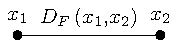
\includegraphics[scale=1]{images/d0.pdf}} \qquad
%      \subfigure []{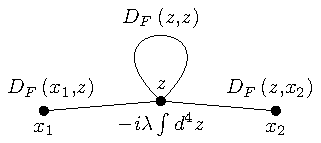
\includegraphics[scale=1]{images/d1.pdf}} \qquad
%      \subfigure [] {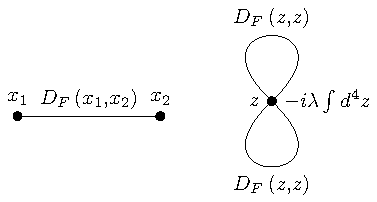
\includegraphics[scale=1]{images/d2.pdf}} \qquad
%     }
%    \caption[Feynman diagrams for the Numerator N$(\lambda^1)$ = $Z_0$A + $Z_0$B + $Z_0$C.]
%    {Feynman diagrams for N$(\lambda^1)$ = $Z_0$A + $Z_0\frac{12}{4!}$B + $Z_0\frac{3}{4!}$C.}
%    \label{fig:feynfullprop}
%\end{figure}
%The denominator is a normalization that serves to eliminate $Z_0$ and the disconnected diagrams with vacuum fluctuations like C. It removes the contributions where the vacuum fluctuates independently from the process of interest \cite{peskin}. Finally, the propagator for the fully interacting theory up to first order in $\lambda$ is 
%\begin{equation}
%\bra{0}\Phi(x_2)\Phi(x_1)\ket{0}_{\lambda^1} = A + \frac{12}{4!}B = \mathcal{D}_F(x_2,x_1) + 
%\frac{12}{4!}(-i\lambda)\int_{-\infty}^{\infty} d^4z \mathcal{D}_F(x_2,z) \mathcal{D}_F(x_1,z) \mathcal{D}_F(z,z).
%\end{equation}
%The factors out front are called symmetry factors and provide a weight for each diagram. In this theory, the symmetry factor for a diagram is the number of nondegenerate ways to place pairs of points into the propagators multiplied by a factor of by $\frac{1}{4!}$ for every interaction vertex. 
%
%The Feynman rules for a theory can be used to build the perturbation series for any process, and this is why they are so ubiquitous. Any n-point correlation function is the weighted\footnote{The weights are the symmetry factors.} sum of all possible diagrams with n external points -- excluding those with disconnected vacuum fluctuations. For $2 \rightarrow 2$ scattering, the correlation function to first order requires the six diagrams shown in Figure \ref{fig:feyn2-2}. 
%\begin{figure}[h!]
%  \centering
%  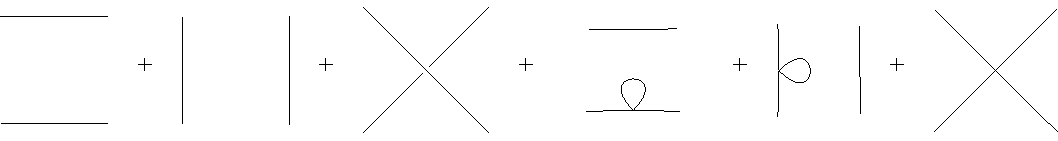
\includegraphics[width=4in]{images/phi4_2-2_scattering.pdf}
%  \caption
%   {The Feynman diagrams for $\bra{0}\Phi(x_4)\Phi(x_3)\Phi(x_2)\Phi(x_1)\ket{0}_{\lambda^1}$ representing the matrix element for $2\rightarrow 2$ scattering up to first order.}
%  \label{fig:feyn2-2}
%\end{figure}
%The first three diagrams are of the form A*A, and these represent the three ways to put four points into $\mathcal{D}_F\mathcal{D}_F$. The next two terms are of the form A*B, and the last one is a new diagram where the particles actually scatter instead of propagating separately. And the last term is built from the following factors: the interaction vertex provides a factor of $-i\lambda\int d^4z$ and the four propagators provide a factor of $\mathcal{D}_F(x_1,z)\mathcal{D}_F(x_2,z)\mathcal{D}_F(x_3,z)\mathcal{D}_F(x_4,z)$. The symmetry factor is $1 = \frac{4!}{4!}$ with the $\frac{1}{4!}$ from the internal vertex and the 4! for the ways to place the zs among $x_1, x_2, x_3, x_4$. All of this results in a mathematical expression for the last diagram, 
%\begin{equation}
%D = -i\lambda\int d^4z\mathcal{D}_F(x_1,z)\mathcal{D}_F(x_2,z)\mathcal{D}_F(x_3,z)\mathcal{D}_F(x_4,z).
%\end{equation}
%Summing the six diagrams yields the full four point correlation function to first order,
%\begin{equation}
%\begin{split}
%\bra{0}\Phi(x_4)\Phi(x_3)\Phi(x_2)\Phi(x_1)\ket{0}_{\lambda^1} &= \mathcal{D}_F(x_1,x_3)\mathcal{D}_F(x_2,x_4) + \mathcal{D}_F(x_1,x_2)\mathcal{D}_F(x_3,x_4) \\ & + \mathcal{D}_F(x_1,x_4)\mathcal{D}_F(x_2,x_3) \\ 
% &+ \mathcal{D}_F(x_1,x_3)\frac{12}{4!}(-i\lambda)\int_{-\infty}^{\infty} d^4z \mathcal{D}_F(x_2,z) \mathcal{D}_F(x_4,z) \mathcal{D}_F(z,z) \\
% &+ \mathcal{D}_F(x_2,x_4)\frac{12}{4!}(-i\lambda)\int_{-\infty}^{\infty} d^4z \mathcal{D}_F(x_1,z) \mathcal{D}_F(x_3,z) \mathcal{D}_F(z,z) \\
% &+ -i\lambda\int d^4z\mathcal{D}_F(x_1,z)\mathcal{D}_F(x_2,z)\mathcal{D}_F(x_3,z)\mathcal{D}_F(x_4,z).
%\end{split}
%\end{equation}
%The Feynman rules for the actual interactions of the Standard Model are derived from the interacting Lagrangians in a similar way. The Feynman diagrams use the appropriate $\mathcal{D}_F$ propagators for the lines and the right coupling factors for the vertices. Different styles of lines are used in the diagrams to represent the different types of propagators. 

%%%%%%%%%%%%%%%%%%%%%%%%%%%%%%%%%%%%%%%%%%%%%%%%%%%%%%%%%%%%%%%%%%%%%%%%%%%
\section{The Standard Model Higgs and the LHC}

The SM Higgs interacts with the massive particles of the SM and even with the massless gluons and photons through second order processes. As such, it can be produced by colliding certain combinations of these particles, and it can decay into them as well. At a particle collider like the LHC, the number of particles expected for a certain process is given by the cross section times the integrated luminosity, $N = \sigma_i*L$. The cross section is proportional to the probability for a production process and consequently, describes how likely a collision attempt is to produce some particle(s) of interest. The luminosity roughly describes the density and the frequency of the incoming particles. Some of the Higgs cross sections for 14 TeV proton-proton collisions are shown in Figure \ref{fig:hprodcross}. 

\begin{figure}[h!]
  \centering
  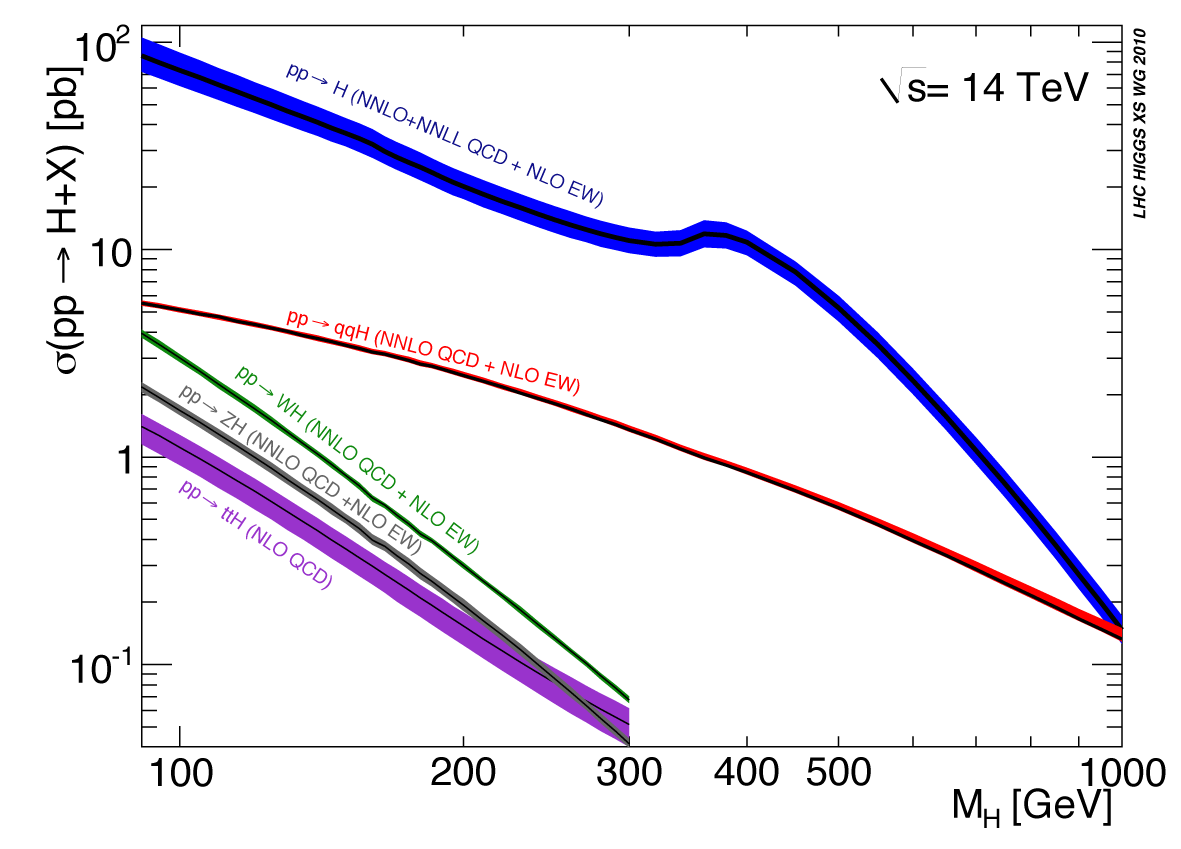
\includegraphics[width=5in]{images/14TeV_higgs_cross_sections.png}
  \caption
   {The highest production mode cross sections for the SM Higgs at 14 TeV \cite{crossbranchplots}}
  \label{fig:hprodcross}
\end{figure}

The Higgs cross sections are functions of the mass of the Higgs as well as the energy of the collisons. For a given collision energy, as in Figure \ref{fig:hprodcross}, the cross sections decrease as the Higgs mass increases. When a larger portion of the collision energy was used to create the mass of the particle, there is less energy to distribute among the kinematic degrees of freedom and therefore fewer possibilities for distribution. On the other hand, for a specific Higgs mass, the cross section grows with collision energy at the LHC. This constrasts with cross sections involving collisions of fundamental particles, e.g. electron antielectron collisions, due to the fact that the LHC collides protons together. 

Protons behave like a quantum superposition of an infinite number of quark-antiquarks, an infinite number of gluons, and the usual uud. As a consequence, the total momentum of a proton in a collision is divided up amongst these constituents called partons. This experimentally verified phenomena is modeled by the parton distribution function, which describes the number of partons with a given fraction of the total momentum. In general, there are many partons with very little of the momentum, and this behavior implies that the cross section should increase with increasing proton momentum. The minimum energy required to create a particular particle is a constant, and at larger proton momentum, this constant is a smaller fraction of the total proton momentum. With more partons at this smaller fraction, there are effectively more partons colliding with the necessary energy. This effective increase in the density of energetic partons results in a growth of the cross section with collision energy. 

If a SM Higgs is produced, it's predicted to decay in about $10^{-22}$ seconds\footnote{Assuming a 125 GeV SM Higgs boson}, which means that the particle itself can't be directly detected at the LHC, only the the decay products can. The SM decay probabilities for the different products are listed in Figure \ref{fig:hbranch}. These probabilities are determined by the coupling, which for the Higgs is the mass of the particle. With a stronger coupling to more massive particles, the decays to the more massive particles are more probable.
\begin{figure}[h!]
  \centering
  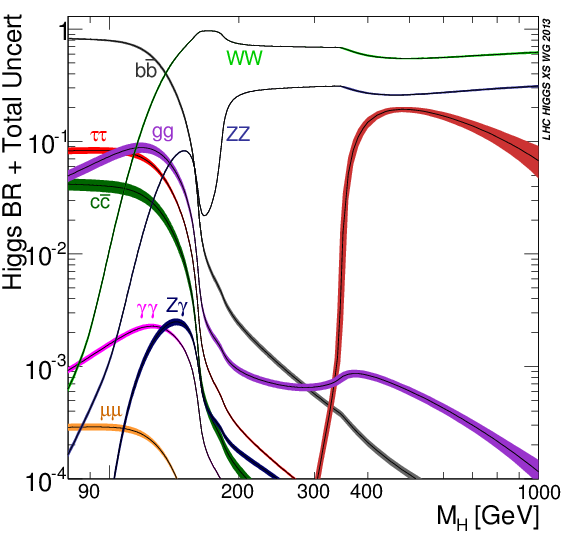
\includegraphics[width=3in]{images/Higgs_BR.png}
  \begin{tabular}{ ll }
    \hline
    Decay & Branching Fraction \\
    \hline
    ${\rm b\bar{b}}$ & 0.57 \\
    $W^+W^-$ & 0.22\\
    gg & 0.085 \\
    ${\rm \tau^+\tau^-}$ & 0.065 \\
    ZZ & 0.027 \\
    ${\rm c\bar{c}}$ & 0.027 \\
    ${\rm \gamma\gamma}$ & 0.0023 \\
    ${\rm Z}\gamma$ & 0.0016 \\
    ${\rm \mu^{+}\mu^{-}}$ & 0.00022 \\
    \hline
  \end{tabular} 
  \caption
{The graphic on the top left presents the SM Higgs branching fractions as functions of mass while the table on the bottom right displays the branching fractions for a 125 GeV SM Higgs \cite{crossbranchplots}.}
  \label{fig:hbranch}
\end{figure}

The muon has the lowest mass \footnote{excluding the photon and gluon} of the particles in Figure ~\ref{fig:hbranch} and consequently H$\rightarrow \mu^{+}\mu^{-}$ has the lowest branching fraction in the set. \footnote{The Higgs also couples to the electron and the first generation quarks but the masses are so light that CMS does not expect to see the SM Higgs in those modes.} The gluons and photons are massless and do not couple to the Higgs at leading order, but through second order processes. Gluons interact with the Higgs through a loop of top quarks, as seen in Figure \ref{fig:hfeynprod}a. The extremely heavy mass of the top quark, about 173 GeV, balances the fact that the loop production is a higher order mechanism. The photons interact with the Higgs through a either a loop of W bosons or a loop of top quarks. 
\begin{figure}[h!]
  \centering
  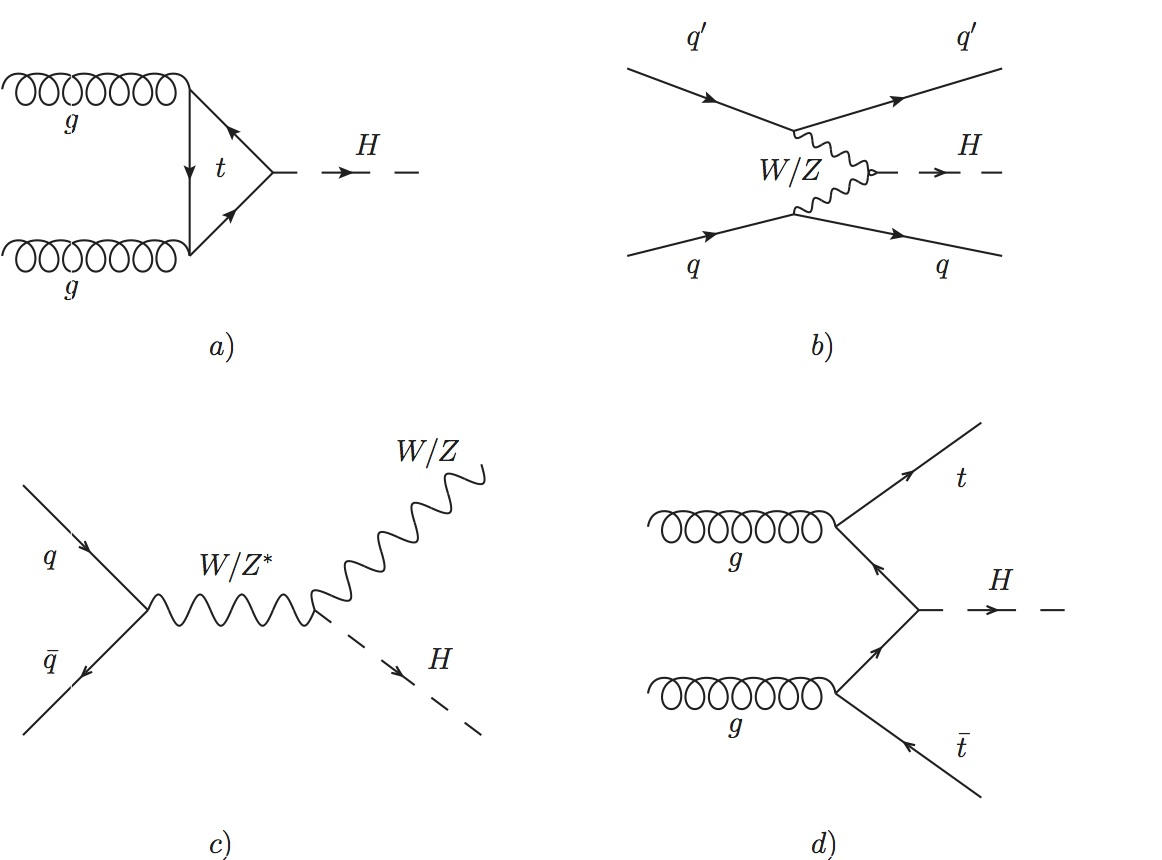
\includegraphics[width=4in]{images/higgs_production_modes.png}
  \caption
   {The SM production modes with the highest cross sections. a) Gluon Gluon Fusion (GGF/ggH) b) Vector Boson Fusion (VBF/qqH) c) Associated Production with a Vector Boson (VH) d) ${\rm t\bar{t}}$H}
  \label{fig:hfeynprod}
\end{figure}
Figure \ref{fig:hfeynprod} shows the highest probability production mechanisms at the LHC. At ${\rm M_{h} = 125}$ GeV, ${\rm \sqrt{s} =}$ 13 TeV, the GGF channel comprises 87\% of the total Higgs production cross section, VBF 7\%, VH 4\%, and ${\rm t\bar{t}}$H 1\% \cite{crossbranchplots}. Besides ${\rm t\bar{t}}$H, the process q + $\bar{q} \rightarrow$ H isn't considered due to its low cross section. The low masses of these other quarks suppress the process. 

Colliding protons full of quarks and gluons results in many quark-gluon (qg) scattering events like the one in Figure \ref{fig:qg}. Quarks and gluons are detected at CMS as collimated jets of energy deposition and not single particles with well defined tracks. Because of this, the different quarks and gluons are difficult to differentiate from one another, and it's difficult to differentiate the quark/gluon Higgs decays from this large background. 
\begin{figure}[h!]
\label{fig:qg}
  \centering
  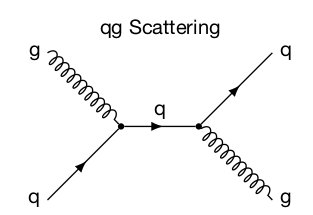
\includegraphics[width=2in]{images/qg_scattering.png}
  \caption
   {The quark-gluon background looks very similar to the GGF production channel when the Higgs decays to two jets. Protons are made of quarks and gluons so this process is extremely common in proton colliders like the LHC.}
  \label{fig:feynqg}
\end{figure}
The Higgs decay to b-quarks is an exception as the b-quark upon production forms a reasonably long lived hadron, which travels from the initial collision point and then decays. In this way, jets that come from displaced vertices are probably b-jets and these events can be collected for study without collecting the majority of the enormous qg background. The relative clarity over the qg background makes $H\rightarrow b\bar{b}$ an important and viable process that allows scientists at the LHC to study the Higgs coupling to fermions and to third generation quarks in particular. The other viable decays to study are those with isolated lepton or photon final states that distinguish them from the overwhelming jet background. 
%\begin{figure}[h!]
%  \centering
%  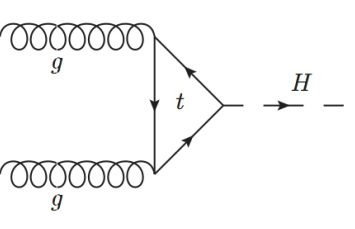
\includegraphics[width=1.5in]{images/ggf.png}
%  \caption
%   {The Feynman diagram for two gluons fusing into a Higgs. There are three vertices and this is a third order diagram. Two vertices involve the strong force and one vertex involves the Higgs coupling. The matrix element for this diagram would have two factors of the strong force coupling and one factor for the Higgs coupling which involves the mass of the top quark.}
%  \label{fig:feynggf}
%\end{figure}
